\documentclass[12pt]{article}

\usepackage[german]{babel}
\usepackage{amsmath}
\usepackage{amssymb} % to display symbols for real numbers, integers etc. Usage: \mathbb{R}
\usepackage{graphicx}
\usepackage{listings} % to display programming code
%\usepackage[ngerman]{babel}
\usepackage{color}
\usepackage{relsize} % to display scaled math symbols (big summation symbol etc.)
\usepackage{textcomp}

\DeclareGraphicsExtensions{.pdf,.jpeg,.png}
\definecolor{listinggray}{gray}{0.9}
\definecolor{lbcolor}{rgb}{0.9,0.9,0.9}
\lstset{ % to display programming code in nice colors
	backgroundcolor=\color{lbcolor},
	tabsize=4,
	rulecolor=,
	language=matlab,
		basicstyle=\scriptsize, %for extra small font size
        upquote=true,
        aboveskip={1.5\baselineskip},
        columns=fixed,
        showstringspaces=false,
        extendedchars=true,
        breaklines=true,
        prebreak = \raisebox{0ex}[0ex][0ex]{\ensuremath{\hookleftarrow}},
		frame=single, %draw frame
        showtabs=false,
        showspaces=false,
        showstringspaces=false,
        identifierstyle=\ttfamily,
        keywordstyle=\color[rgb]{0,0,1},
        commentstyle=\color[rgb]{0.133,0.545,0.133},
        stringstyle=\color[rgb]{0.627,0.126,0.941},
        numbers=left,
        stepnumber=1,
        firstnumber=1,
        numberfirstline=true,
        linewidth=14cm,
}

\title{Uebungsblatt 2\\ \glqq Mustererkennung\grqq}
\author{J. Cavojska, N. Lehmann}
\date{05.05.2015}
\begin{document}
\maketitle
%\renewcommand{\contentsname}{Table of Contents}
%\tableofcontents

\section{Aufgabe 1 - KNN}
\textit{Schreiben Sie in matlab oder octave ein Script, das die Datensätze aus ​chickwts\_testing.csv​ anhand der Datensätze aus chickwts\_training.csv​ mit dem K­NN-­Algorithmus klassifiziert und die Konfusionsmatrix und Klassifikationsgüte (korrekt klassifizierte Individuen geteilt durch Gesamtzahl der Individuen) ausgibt. Geben Sie die Konfusionsmatrix und Klassifikationsgüte jeweils für K = 1, 3 und 5 an.}\\
\\
\textit{Notiz:} Fuer die Aufg. 1 haben wir Trainingsdaten verwendet, von denen duplikate Eintraege vorher entfernt wurden (Huehner, die das gleiche Gewicht UND die gleiche Futterklasse hatten).\\


\subsection{Code fuer Klassifikator, Konfusionsmatrix und Klassifikationsguete}
\begin{lstlisting}[language=Python]
% Spalte 1 = Huhn-ID, Spalte 2 = Gewicht, Spalte 3 = Futterklasse

A = load('chickwts_training.csv');
A_Sorted = sortrows(A,2); % nach Gewichten sortieren
A_Training = A(:,2:3);
U = unique(A_Training,'rows');
zeilen = size(U,1);
B = load('chickwts_testing.csv');
B_Testing = B(:,2:3);

alle_k = [1 3 5];
for k=alle_k
  fprintf('k = %i\n',k)
  dists = zeros(2*k - 1, 2); %  (2*k-1)x2-Matrix mit den 5 Kandidat-Nachbarn 
  % um unser Eingabehuhn h herum. 3 von diesen 5 Nachbarn sind die 3 nearest 
  % neighbors unseres Huhns. 1. Spalte enthaelt die Distanzen, 2. Spalte enthaelt
  % die Klassen dieser Nachbarn.
  
  C = []; % Ergebnismatrix
  for zeilenindex_testdaten = 1:size(B_Testing,1)
    h = B_Testing(zeilenindex_testdaten, 1); % unser Testhuhn
    % Huhn 'treffer' finden, das unserem Huhn h am naechsten ist:
    treffer = -1;
    trefferZeile = -1; % Zeile, in welcher wir das 'treffer'-Huhn gefunden haben
    if h < U(1,1)
      treffer = U(1,2);
      trefferZeile = 1;
    elseif h > U(zeilen,1)
      treffer = U(zeilen,2);
      trefferZeile = zeilen;
    else
    
      for z = 1:zeilen
        if h == U(z, 1)
          treffer = U(z, 2);
          trefferZeile = z;
          break
        elseif h < U(z,1)
          dist1 = abs(U(z-1, 1) - h);
          dist2 = abs(U(z, 1) - h);
          if dist1 <= dist2
            treffer = U(z-1,2);
            trefferZeile = z;
            break
          else
            treffer = U(z,2);
            trefferZeile = z;
            break
          end
        end
      end  
    end
    % Wir haben unseren 'treffer' gefunden. Nun entscheiden wir, welche Huehner um ihn herum unsere k naechsten Nachbarn sind.
    if k == 1
      most_frequent_neighbor_class = treffer;
    elseif k > 1
      offset = 0;
      if trefferZeile < k
        offset = k - trefferZeile; % 3-1 = 2
      elseif trefferZeile > zeilen - k + 1
        offset = zeilen - k + 1 - trefferZeile; % 10-3+1-10 = -2
      end
      dists = U(trefferZeile-(k-1)+offset:trefferZeile+(k-1)+offset, :); % aus U ein Fenster der Laenge 2*k-1 um 'treffer' herum ausschneiden
      dists = [abs((dists(:,1)) - h), dists(:,2)]; % Gewichte ersetzen durch Distanzen der Gewichte zu h.
      dists = sortrows(dists,1); % nach Gewicht-Distanzen sortieren
      k_neighbors_classes = dists(1:k, 2); % die Klassen der k Nachbarn mit den kleinsten Gewicht-Distanzen holen
      most_frequent_neighbor_class = mode(k_neighbors_classes); % findet die haeufigste Klasse in k_neighbors_classes
    end
    
    % Ergebnismatrix C: 1. Spalte: Gewicht, 2. Spalte: Futterklasse (Testdaten), 3. Spalte: Futterklasse (Trainingsdaten)
    tmpVector = [B_Testing(zeilenindex_testdaten, 1), B_Testing(zeilenindex_testdaten, 2), most_frequent_neighbor_class];
      C = vertcat(C,tmpVector);
      
  end % end of for each test chicken
  
  % Konfusionsmatrix
  knownClass = C(:, 2);
  predictedClass = C(:, 3);
  confusionMatrix = confusionmat(knownClass, predictedClass)

  % Klassifikationsguete
  alle = size(C, 1);
  korrekt_vorhergesagt = 0;
  for z = 1:alle
    if C(z, 2) == C(z, 3)
      korrekt_vorhergesagt = korrekt_vorhergesagt + 1;
    end
  end
  Klassifikationsguete = korrekt_vorhergesagt / alle
end % end of for k in 1, 3, 5

\end{lstlisting}
 
\subsubsection{Konfusionsmatrizen und Klassifikationsgueten}
Rows: actual classes, Columns: predicted classes\\
\\
k = 1\\
confusionMatrix =\\
\begin{tabular}{ c c c c c c }
 3 & 3 & 1 & 0 & 3 & 0\\
 5 & 6 & 1 & 0 & 0 & 0\\
 2 & 2 & 4 & 3 & 3 & 0\\
 0 & 1 & 1 & 6 & 2 & 2\\
 3 & 1 & 1 & 4 & 1 & 1\\
 0 & 3 & 3 & 3 & 0 & 3\\
\end{tabular}\\
Klassifikationsguete = 0.3239\\

k = 3\\
confusionMatrix =\\
\begin{tabular}{ c c c c c c }
 7 & 0 & 2 & 0 & 1 & 0\\
 6 & 4 & 0 & 0 & 2 & 0\\
 3 & 0 & 6 & 2 & 3 & 0\\
 1 & 1 & 2 & 7 & 0 & 1\\
 4 & 1 & 1 & 4 & 1 & 0\\
 0 & 3 & 3 & 3 & 0 & 3\\
\end{tabular}\\
Klassifikationsguete = 0.3944\\

k = 5\\
confusionMatrix =\\
\begin{tabular}{ c c c c c c }
 7 & 0 & 2 & 0 & 1 & 0\\
 6 & 3 & 0 & 1 & 2 & 0\\
 2 & 1 & 7 & 1 & 3 & 0\\
 0 & 0 & 3 & 7 & 1 & 1\\
 2 & 2 & 1 & 5 & 1 & 0\\
 0 & 1 & 3 & 3 & 0 & 5\\
\end{tabular}\\
Klassifikationsguete = 0.4225\\



\section{Aufgabe 2 - Normalverteilung}
\textit{Notiz:} Fuer Aufgabe 2 haben wir die Originaldaten genommen, ohne die Duplikate vorher zu entfernen.\\
\\
\textit{a) Berechnen Sie die ​Normalverteilung​ (Erwartungswert und Varianz) über den Gewichten jeweils für alle 6 Futterklassen sowie die ​ A­priori­Wahrscheinlichkeit​ für jede der 6 Futterklassen anhand der Werte aus ​chickwts\_training.csv​.}\\
\\
\subsection{Code fuer Aufg. 2 a)}
\begin{lstlisting}[language=Python]
% Berechnungen fuer die 6 Futtermittel FM0..FM5:

FM0_matrix = A_Training(A_Training(:,2)==0,1);
FM1_matrix = A_Training(A_Training(:,2)==1,1);
FM2_matrix = A_Training(A_Training(:,2)==2,1);
FM3_matrix = A_Training(A_Training(:,2)==3,1);
FM4_matrix = A_Training(A_Training(:,2)==4,1);
FM5_matrix = A_Training(A_Training(:,2)==5,1);

% Erwartungswert/Mittelwert berechnen
FM0_mean = mean(FM0_matrix);
FM1_mean = mean(FM1_matrix);
FM2_mean = mean(FM2_matrix);
FM3_mean = mean(FM3_matrix);
FM4_mean = mean(FM4_matrix);
FM5_mean = mean(FM5_matrix);

% Varianz
FM0_var = var(FM0_matrix);
FM1_var = var(FM1_matrix);
FM2_var = var(FM2_matrix);
FM3_var = var(FM3_matrix);
FM4_var = var(FM4_matrix);
FM5_var = var(FM5_matrix);

% Standardabweichungen
FM0_std = std(FM0_matrix);
FM1_std = std(FM1_matrix);
FM2_std = std(FM2_matrix);
FM3_std = std(FM3_matrix);
FM4_std = std(FM4_matrix);
FM5_std = std(FM5_matrix);

% A Priori Wahrscheinlickeit berechnen
FM0_apriori = length(FM0_matrix) / length(A_Training)
FM1_apriori = length(FM1_matrix) / length(A_Training)
FM2_apriori = length(FM2_matrix) / length(A_Training)
FM3_apriori = length(FM3_matrix) / length(A_Training)
FM4_apriori = length(FM4_matrix) / length(A_Training)
FM5_apriori = length(FM5_matrix) / length(A_Training)
\end{lstlisting}

\subsection{Ergebnisse fuer Aufg. 2 a)}

FM0\_mean = 165.7200\\
FM1\_mean = 217.9167\\
FM2\_mean = 244.6429\\
FM3\_mean = 325.6000\\
FM4\_mean = 281.8182\\
FM5\_mean = 326.9333\\
\\
FM0\_var = 2.0801e+03\\
FM1\_var = 3.8649e+03\\
FM2\_var = 3.6319e+03\\
FM3\_var = 3.2483e+03\\
FM4\_var = 5.3364e+03\\
FM5\_var = 4.8296e+03\\
\\
FM0\_std = 45.6079\\
FM1\_std = 62.1682\\
FM2\_std = 60.2656\\
FM3\_std = 56.9937\\
FM4\_std = 73.0505\\
FM5\_std = 69.4952\\
\\
FM0\_apriori = 0.1408\\
FM1\_apriori = 0.1690\\
FM2\_apriori = 0.1972\\
FM3\_apriori = 0.1690\\
FM4\_apriori = 0.1549\\
FM5\_apriori = 0.1690\\
\\
\begin{lstlisting}[language=Python]
\% PDFs plotten (in einer Grafik)\\
X = A_Training(:,1);\\
x = min(X):max(X); \% Abschnitt auf der x-Achse, der geplottet werden soll\\
\\
\% PDFs berechnen\\
\% pdf(Art von Verteilung, Abschnitt auf x-Achse, mean, std)\\
FM0_pdf = pdf('Normal',x,FM0_mean, FM0_std);\\
FM1_pdf = pdf('Normal',x,FM1_mean, FM1_std);\\
FM2_pdf = pdf('Normal',x,FM2_mean, FM2_std);\\
FM3_pdf = pdf('Normal',x,FM3_mean, FM3_std);\\
FM4_pdf = pdf('Normal',x,FM4_mean, FM4_std);\\
FM5_pdf = pdf('Normal',x,FM5_mean, FM5_std);\\
\\
P1 = plot(x,FM0_pdf,x,FM1_pdf,x,FM2_pdf,x,FM3_pdf,x,FM4_pdf,x,FM5_pdf);\\
\end{lstlisting}
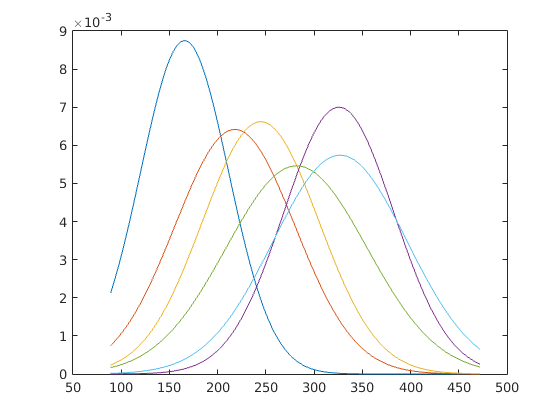
\includegraphics{ueb02_pdf_Aufg2a.png}



\textit{b) Plotten Sie die A­-posteriori-­Wahrscheinlichkeitsdichtefunktion p(Futterklasse | Gewicht) für alle 6 Futterklassen zusammen in einem Diagramm. Verwenden Sie dabei die Werte aus a).}\\
\\
\begin{lstlisting}[language=Python]
FM0_aposteriori = FM0_pdf * FM0_apriori;
FM1_aposteriori = FM1_pdf * FM1_apriori;
FM2_aposteriori = FM2_pdf * FM2_apriori;
FM3_aposteriori = FM3_pdf * FM3_apriori;
FM4_aposteriori = FM4_pdf * FM4_apriori;
FM5_aposteriori = FM5_pdf * FM5_apriori;
% PDFs plotten (in einer Grafik)
P2 = plot(x,FM0_aposteriori,x,FM1_aposteriori,x,FM2_aposteriori,x,FM3_aposteriori,x,FM4_aposteriori,x,FM5_aposteriori);
\end{lstlisting}
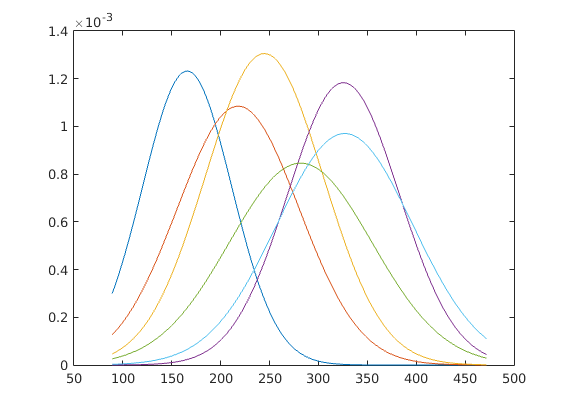
\includegraphics{ueb02_pdf_Aufg2b_gefragt.png}


\textit{c) Klassifizieren Sie die Hühner in chickwts\_testing.csv​ ​mit einem Bayes­Klassifikator anhand ihres Gewichtes in die 6 Futterklassen. Verwenden Sie dabei die Werte bzw. Wahrscheinlichkeitsdichtefunktionen aus a) und b). Geben Sie die die Konfusionsmatrix und Klassifikationsgüte aus.}\\
\\
\begin{lstlisting}[language=Python]
D = [];
for huhnIndex = 1:size(B_Testing,1)
  h = B_Testing(huhnIndex, 1);
  fm0pre = pdf('Normal', h, FM0_mean, FM0_std) * FM0_apriori;
  fm1pre = pdf('Normal', h, FM1_mean, FM0_std) * FM1_apriori;
  fm2pre = pdf('Normal', h, FM2_mean, FM0_std) * FM2_apriori;
  fm3pre = pdf('Normal', h, FM3_mean, FM0_std) * FM3_apriori;
  fm4pre = pdf('Normal', h, FM4_mean, FM0_std) * FM4_apriori;
  fm5pre = pdf('Normal', h, FM5_mean, FM0_std) * FM5_apriori;
  
  [maxValue, indexAtMaxValue] = max([fm0pre,fm1pre,fm2pre,fm3pre,fm4pre,fm5pre]);
  
  if (maxValue == fm0pre)
    tmpVector = [B_Testing(huhnIndex,1),B_Testing(huhnIndex,2),0];
    D = vertcat(D,tmpVector);
  elseif (maxValue == fm1pre)
    tmpVector = [B_Testing(huhnIndex,1),B_Testing(huhnIndex,2),1];
    D = vertcat(D,tmpVector);
  elseif (maxValue == fm2pre)
    tmpVector = [B_Testing(huhnIndex,1),B_Testing(huhnIndex,2),2];
    D = vertcat(D,tmpVector);  
  elseif (maxValue == fm3pre)
    tmpVector = [B_Testing(huhnIndex,1),B_Testing(huhnIndex,2),3];
    D = vertcat(D,tmpVector);
  elseif (maxValue == fm4pre)
    tmpVector = [B_Testing(huhnIndex,1),B_Testing(huhnIndex,2),4];
    D = vertcat(D,tmpVector);
  else
    tmpVector = [B_Testing(huhnIndex,1),B_Testing(huhnIndex,2),5];
    D = vertcat(D,tmpVector);
  end
end % end of for each h

% Konfusionsmatrix
  knownClass = D(:, 2);
  predictedClass = D(:, 3);
  confusionMatrix = confusionmat(knownClass, predictedClass)

  % Klassifikationsguete
  alle = size(D, 1);
  korrekt_vorhergesagt = 0;
  for z = 1:alle
    if D(z, 2) == D(z, 3)
      korrekt_vorhergesagt = korrekt_vorhergesagt + 1;
    end
  end
  Klassifikationsguete = korrekt_vorhergesagt / alle
\end{lstlisting}
\textbf{Konfusionsmatrix und Klassifikationsguete}\\
\\
confusionMatrix =\\
\begin{tabular}{ c c c c c c }
 8 & 1 & 1 & 0 & 0 & 0\\
 4 & 2 & 5 & 1 & 0 & 0\\
 2 & 2 & 7 & 1 & 0 & 2\\
 0 & 0 & 1 & 3 & 2 & 6\\
 1 & 1 & 4 & 3 & 0 & 2\\
 0 & 1 & 2 & 1 & 1 & 7\\
\end{tabular}\\
Klassifikationsguete = 0.3803

\end{document}